% =====================================================================
%  HEL-Net Explained -- a step-by-step, beginner-friendly walkthrough
%  Source: "HEL-Net, Decoded" (Paper Decode) of
%  Wu, Xia, Song, Lan, Image and Vision Computing 166 (2026) 105879
%  Compile:  pdflatex hel_net_explained.tex   (run twice for the TOC)
% =====================================================================
\documentclass[11pt,a4paper]{article}

\usepackage[T1]{fontenc}
\usepackage[utf8]{inputenc}
\usepackage{lmodern}
\usepackage[scaled=0.92]{helvet}
\usepackage[margin=2.2cm,headheight=14pt]{geometry}
\usepackage{amsmath,amssymb,bm}
\usepackage{booktabs,tabularx,array,multirow}
\usepackage{xcolor}
\usepackage{enumitem}
\usepackage{fancyhdr}
\usepackage{titlesec}
\usepackage{pifont}
\usepackage[most]{tcolorbox}
\usepackage{tikz}
\usetikzlibrary{arrows.meta,positioning,fit,calc,shapes.geometric,backgrounds}
\usepackage{pgfplots}
\pgfplotsset{compat=1.17}
\usepackage[colorlinks=true,linkcolor=navy,urlcolor=navy]{hyperref}

% ---------- colours ----------
\definecolor{navy}{HTML}{0E2240}
\definecolor{gold}{HTML}{C9A227}
\definecolor{goldlight}{HTML}{F7EFD6}
\definecolor{navylight}{HTML}{E6ECF5}
\definecolor{okgreen}{HTML}{2E7D32}
\definecolor{badred}{HTML}{B3261E}
\definecolor{redlight}{HTML}{FBEAEA}
\definecolor{teal}{HTML}{00796B}
\definecolor{teallight}{HTML}{E0F2F1}
\definecolor{purple}{HTML}{5E35B1}
\definecolor{purplelight}{HTML}{EDE7F6}

\newcommand{\cmark}{\textcolor{okgreen}{\ding{51}}}
\newcommand{\xmark}{\textcolor{badred}{\ding{55}}}

% ---------- headings ----------
\setcounter{secnumdepth}{0}
\titleformat{\section}{\sffamily\Large\bfseries\color{navy}}
  {}{0em}{{\color{gold}\rule[-0.15em]{0.35em}{1.1em}}\hspace{0.5em}}
  [{\color{gold}\titlerule[0.8pt]}]
\titleformat{\subsection}{\sffamily\large\bfseries\color{navy}}
  {}{0em}{}
\titleformat{\subsubsection}{\sffamily\normalsize\bfseries\color{navy}}{}{0em}{}

\pagestyle{fancy}
\fancyhf{}
\fancyhead[L]{\sffamily\small\color{navy}HEL-Net, explained step by step}
\fancyhead[R]{\sffamily\small\color{gold}\leftmark}
\fancyfoot[C]{\sffamily\small\thepage}
\renewcommand{\headrulewidth}{0.4pt}
\renewcommand{\sectionmark}[1]{\markboth{#1}{}}

\setlist{itemsep=2pt,topsep=4pt}
\setlength{\parskip}{4pt}
\setlength{\parindent}{0pt}

% ---------- boxes ----------
\newtcolorbox{idea}[1][Big idea]{enhanced,colback=navylight,colframe=navy,
  fonttitle=\sffamily\bfseries,title=#1,arc=2pt,boxrule=0.6pt}
\newtcolorbox{analogy}[1][Everyday analogy]{enhanced,colback=goldlight,colframe=gold!85!black,
  fonttitle=\sffamily\bfseries,title=#1,arc=2pt,boxrule=0.6pt}
\newtcolorbox{worked}[1][Worked example]{enhanced,colback=teallight,colframe=teal,
  fonttitle=\sffamily\bfseries,title=#1,arc=2pt,boxrule=0.6pt}
\newtcolorbox{careful}[1][Careful reader's note]{enhanced,colback=redlight,colframe=badred,
  fonttitle=\sffamily\bfseries,title=#1,arc=2pt,boxrule=0.6pt}
\newtcolorbox{ethics}[1][AI ethics corner]{enhanced,colback=purplelight,colframe=purple,
  fonttitle=\sffamily\bfseries,title=#1,arc=2pt,boxrule=0.6pt}
\newtcolorbox{recap}{enhanced,colback=white,colframe=navy,
  fonttitle=\sffamily\bfseries,title=Step recap,arc=2pt,boxrule=0.6pt,
  borderline west={3pt}{0pt}{gold}}

% ---------- tikz styles ----------
\tikzset{
  blk/.style={draw=navy,rounded corners=2pt,align=center,font=\sffamily\scriptsize,
              minimum height=7mm,inner sep=3pt,fill=white},
  mamba/.style={blk,fill=navylight},
  unet/.style={blk,fill=goldlight},
  dark/.style={blk,fill=navy,text=white},
  arr/.style={-{Stealth[length=2mm]},thick,navy},
  darr/.style={-{Stealth[length=2mm]},thick,gold!80!black,dashed},
}

% =====================================================================
\begin{document}

% ---------------------------- title page -----------------------------
\begin{titlepage}
\begin{tikzpicture}[remember picture,overlay]
  \fill[navy] (current page.north west) rectangle ([yshift=-9.5cm]current page.north east);
  \fill[gold] ([yshift=-9.5cm]current page.north west) rectangle ([yshift=-9.9cm]current page.north east);
\end{tikzpicture}
\vspace*{0.4cm}
{\sffamily\bfseries\color{gold}\large A STEP-BY-STEP LEARNING GUIDE}\\[0.5cm]
{\sffamily\bfseries\color{white}\fontsize{30}{36}\selectfont HEL-Net, Explained}\\[0.4cm]
{\sffamily\color{white}\large How a team of different neural networks finds four kinds of\\[2pt]
eye-disease lesions in retinal photographs --- told from zero}\\[0.5cm]
{\sffamily\color{white}\small Based on: Wu, Xia, Song, Lan, \emph{``HEL-Net: Heterogeneous Ensemble Learning
for comprehensive diabetic retinopathy multi-lesion segmentation via Mamba-UNet''},\\
Image and Vision Computing 166 (2026) 105879, and the accompanying ``HEL-Net, Decoded'' analysis.}

\vspace{3.2cm}
\begin{idea}[What you will be able to do after reading]
\begin{enumerate}[leftmargin=*]
  \item Explain \textbf{what problem} the paper solves and \textbf{why it is hard}, in plain words.
  \item Walk through the HEL-Net pipeline \textbf{one step at a time}: data augmentation
        $\rightarrow$ coarse map $\rightarrow$ data fusion $\rightarrow$ specialist branches
        $\rightarrow$ feature aggregation $\rightarrow$ loss.
  \item Understand the key maths (Poisson blending, state-space models / Mamba, Dice and IoU)
        through \textbf{small worked numerical examples}.
  \item Read the results tables like a reviewer, spot the \textbf{weak points}, and reflect on the
        \textbf{AI-ethics questions} that medical-AI papers raise.
\end{enumerate}
\end{idea}

\begin{analogy}[How to use this guide]
Every step follows the same rhythm: \textbf{Big idea} (navy) $\rightarrow$ \textbf{Everyday analogy}
(gold) $\rightarrow$ the technical detail $\rightarrow$ a \textbf{Worked example} (teal) $\rightarrow$
a \textbf{Step recap}. Red boxes flag mistakes or ambiguities in the paper; purple boxes are
\textbf{AI ethics} reflections. A self-check quiz with answers is at the end.
\end{analogy}

\vfill
{\sffamily\small\color{navy} Prepared for Dr.\ S.\ Satyanarayana \textbullet{} October 2026}\\
{\sffamily\scriptsize\color{gray} Original explanatory text. Numbers are restated from the paper
for study and critique; all diagrams are original redraws.}
\end{titlepage}

\tableofcontents
\newpage

% =====================================================================
\section{The paper in one minute}
% =====================================================================

\begin{idea}[The whole paper in four sentences]
\begin{enumerate}[leftmargin=*]
\item \textbf{Problem.} Diabetic retinopathy (DR) damages the retina and leaves four kinds of
      tiny marks (``lesions'') that doctors look for; finding all four automatically, pixel by
      pixel, is hard because they differ hugely in size, shape and position, and they are very rare.
\item \textbf{Idea.} Instead of one network that must be good at everything, use a
      \emph{team of different specialists}: a first network draws a rough map, then four
      specialist networks --- each tuned to one lesion type --- refine it.
\item \textbf{Twist.} The specialists are \emph{heterogeneous}: two are classic U-Nets
      (good at small local detail) and two are Mamba-UNets (good at long-range, global context).
      A tiny learned ``voting'' layer combines their answers.
\item \textbf{Evidence.} On two public datasets (IDRiD and DDR) HEL-Net beats 14 earlier methods on
      most metrics, e.g.\ mean Dice $67.40\%$, mean IoU $51.99\%$, mean AUPR $69.52\%$ on IDRiD.
\end{enumerate}
\end{idea}

\begin{analogy}[A hospital analogy]
Think of a junior doctor who first glances at the photograph and circles ``suspicious areas''
(\textbf{Stage 1}). The photo plus these circles is then sent to four consultants --- one per
lesion type (\textbf{Stage 2}). Some consultants are detail-oriented (U-Net), others look at the
whole picture (Mamba-UNet). Finally a chairperson decides, lesion by lesion, \emph{whose opinion to
trust most} (\textbf{Feature Aggregation Block}).
\end{analogy}

\subsection*{The paper's anatomy}
\begin{center}
\small
\begin{tabular}{@{}llcc@{}}
\toprule
Section & What it does & Pages & Figs / Tables\\
\midrule
Abstract + 1 Introduction & Problem, gap, proposal, contributions & 1.6 & 1 / -- \\
2 Related work & CNN / Transformer / Mamba families & 1.2 & -- \\
3 Methodology & Augmentation, HEL-Net, Mamba-UNet, loss & 3.5 & 4 / 1\\
4 Experiments & Data, comparisons, statistics, ablations, cost & 6.2 & 6 / 10\\
5 Conclusion & Summary, limitation, future work & 0.6 & -- \\
\bottomrule
\end{tabular}
\end{center}
Notice that almost half the paper is \emph{evidence}. In applied medical imaging, the experiments
section is what convinces reviewers.

% =====================================================================
\section{Background you need first}
% =====================================================================
This section builds the vocabulary. If you already know a concept, skip its paragraph.

\subsection{Diabetic retinopathy and its four lesions}
A fundus photograph is a colour picture of the back of the eye (the retina). In DR, damaged
blood vessels create four lesion types:

\begin{center}
\small
\begin{tabularx}{\linewidth}{@{}l l X l@{}}
\toprule
Code & Name & What it looks like & Typical size\\
\midrule
\textbf{MA} & Microaneurysm & tiny red dots --- small bulges in capillaries & a few pixels\\
\textbf{HE} & Haemorrhage & dark-red blots of leaked blood & small to large\\
\textbf{EX} & Hard exudate & bright yellow, sharp-edged deposits of fat/protein & small to large clusters\\
\textbf{SE} & Soft exudate (cotton-wool spot) & pale, fluffy white patches & medium\\
\bottomrule
\end{tabularx}
\end{center}

\subsection{What is ``segmentation''?}
\begin{idea}[Classification vs.\ segmentation]
\emph{Classification} answers ``Does this image contain DR?'' (one label per image).
\emph{Segmentation} answers ``\textbf{Which pixels} belong to each lesion?'' (one label per pixel).
Multi-lesion segmentation outputs \textbf{four probability maps} --- one per lesion type --- each the
same size as the image.
\end{idea}

\subsection{The three model families}
\begin{description}[leftmargin=0pt,style=nextline]
\item[CNN / U-Net (2015)] A convolutional network shaped like a ``U'': an \emph{encoder} shrinks the image
  and extracts features; a \emph{decoder} grows it back to full size; \emph{skip connections} copy fine
  detail across. Strength: sharp local detail. Weakness: each filter only ``sees'' a small window,
  so understanding the whole retina at once is hard.
\item[Transformer] Uses \emph{self-attention}: every image patch compares itself with every other patch.
  Strength: global context. Weakness: cost grows with the \textbf{square} of the number of patches,
  $\mathcal{O}(L^2)$.
\item[Mamba / State-Space Model (SSM)] Reads the patches as a sequence and carries a running
  ``memory'' $h_t$ forward, like reading a book and keeping notes. Strength: long-range context at
  \textbf{linear} cost $\mathcal{O}(L)$. \emph{Mamba-UNet} is a U-Net whose building blocks are Mamba
  blocks.
\end{description}

\begin{worked}[Why linear vs.\ quadratic matters]
HEL-Net resizes images to $800\times800$ and cuts them into $4\times4$ patches:
\[
L=\frac{800}{4}\times\frac{800}{4}=200\times200=40\,000 \text{ tokens}.
\]
Self-attention would compute $L^2 = 1.6\times10^{9}$ pairwise scores per head per layer.
A Mamba scan does work proportional to $L=4\times10^{4}$ --- roughly \textbf{40\,000 times less}.
That is why Mamba is attractive for high-resolution medical images.
\end{worked}

\subsection{What is an ensemble, and what makes it ``heterogeneous''?}
An \emph{ensemble} combines several models' predictions, like asking several experts and
voting. \emph{Homogeneous} = all experts have the same architecture.
\emph{Heterogeneous} = experts are \textbf{different kinds} of networks, so they make
\emph{different} mistakes --- and different mistakes cancel better when combined.

\subsection{How segmentation is scored}
Compare the predicted pixels with the doctor-annotated ``ground truth''.
Count \textbf{TP} (lesion pixels found), \textbf{FP} (false alarms) and \textbf{FN} (lesion pixels missed).

\begin{center}
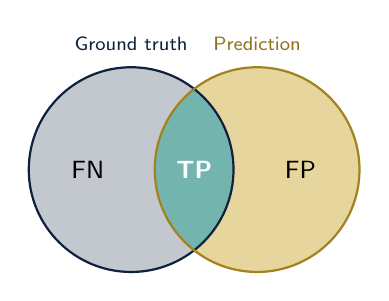
\begin{tikzpicture}
  \fill[navy!25] (0,0) circle (1.3);
  \fill[gold!45] (1.6,0) circle (1.3);
  \begin{scope}\clip (0,0) circle (1.3); \fill[teal!55] (1.6,0) circle (1.3); \end{scope}
  \draw[navy,thick] (0,0) circle (1.3);
  \draw[gold!80!black,thick] (1.6,0) circle (1.3);
  \node[font=\sffamily\small] at (-0.55,0) {FN};
  \node[font=\sffamily\small,text=white] at (0.8,0) {\textbf{TP}};
  \node[font=\sffamily\small] at (2.15,0) {FP};
  \node[font=\sffamily\scriptsize,navy] at (0,1.6) {Ground truth};
  \node[font=\sffamily\scriptsize,gold!70!black] at (1.6,1.6) {Prediction};
\end{tikzpicture}
\end{center}

\[
\text{Dice}=\frac{2\,TP}{2\,TP+FP+FN},\qquad
\text{IoU}=\frac{TP}{TP+FP+FN},\qquad
\text{IoU}=\frac{\text{Dice}}{2-\text{Dice}} .
\]
\textbf{AUPR} (area under the precision--recall curve) summarises performance over \emph{all}
thresholds, so it does not depend on choosing a cut-off such as 0.5. The prefix ``m'' (mDice,
mIoU, mAUPR) means the average over the four lesion types.

\begin{worked}[Dice and IoU on a toy image]
Suppose for one lesion $TP=80$, $FP=10$, $FN=20$ pixels.
\[
\text{Dice}=\frac{160}{160+10+20}=\frac{160}{190}=0.842,\qquad
\text{IoU}=\frac{80}{80+10+20}=\frac{80}{110}=0.727.
\]
Check the identity: $0.842/(2-0.842)=0.842/1.158=0.727$ \cmark.
\textbf{Lesson:} Dice and IoU always rank models the same way, so the paper's AUPR column is the one
that adds genuinely independent evidence.
\end{worked}

\begin{recap}
Four lesions (MA, HE, EX, SE) $\cdot$ per-pixel labelling $\cdot$ U-Net = local, Transformer = global
but expensive, Mamba = global and cheap $\cdot$ heterogeneous ensemble = different experts $\cdot$
Dice / IoU / AUPR measure overlap.
\end{recap}

% =====================================================================
\section{Step 0 --- Why is this problem hard?}
% =====================================================================
The paper names \textbf{two challenges}:

\begin{enumerate}
\item \textbf{Extreme diversity.} An MA may be 3--5 pixels; an exudate cluster may cover a large region.
  One network rarely handles both scales well.
\item \textbf{Local vs.\ global conflict.} Small lesions need fine local detail (CNN strength); big,
  scattered lesions need long-range context (Transformer/Mamba strength). Most models choose one.
\end{enumerate}
A third, hidden challenge is \textbf{class imbalance}:
\begin{center}
\small
\begin{tabular}{@{}lc@{}}
\toprule
Pixel type (IDRiD) & Share of all pixels\\
\midrule
Background (no lesion) & 97.80\%\\
All lesions together & $\approx$ 2.2\%\\
Soft exudates (SE) & 0.19\%\\
Microaneurysms (MA) & 0.10\%\\
\bottomrule
\end{tabular}
\end{center}

\begin{worked}[How rare is 0.10\%?]
An $800\times800$ image has $640\,000$ pixels. $0.10\%$ of that is about \textbf{640 MA pixels}
in the whole image. A lazy network that predicts ``no MA anywhere'' is already $99.9\%$ accurate ---
which is why plain accuracy is useless here and why Dice/IoU/AUPR and weighted losses are used.
\end{worked}

The datasets are also small: \textbf{IDRiD} has 81 images (54 train / 27 test) and \textbf{DDR} has 757
images (383 train / 149 validation / 225 test).

% =====================================================================
\section{The full pipeline at a glance}
% =====================================================================
\begin{center}
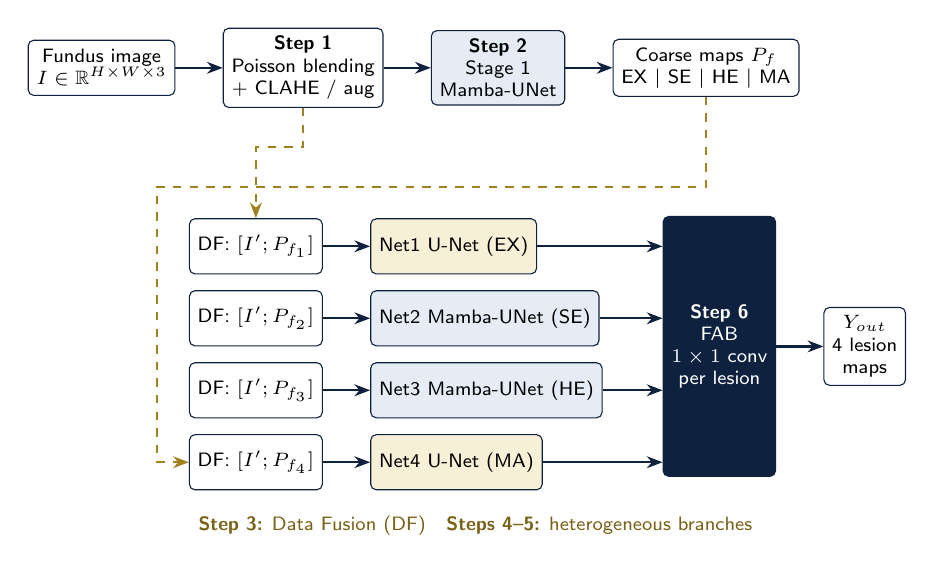
\begin{tikzpicture}[node distance=4mm and 6mm]
  \node[blk] (in) {Fundus image\\$I\in\mathbb{R}^{H\times W\times 3}$};
  \node[blk,right=of in] (aug) {\textbf{Step 1}\\Poisson blending\\+ CLAHE / aug};
  \node[mamba,right=of aug] (s1) {\textbf{Step 2}\\Stage 1\\Mamba-UNet};
  \node[blk,right=of s1] (pf) {Coarse maps $P_f$\\EX $|$ SE $|$ HE $|$ MA};

  \node[blk,below=14mm of aug,xshift=-6mm] (df1) {DF: $[I';P_{f_1}]$};
  \node[blk,below=2mm of df1] (df2) {DF: $[I';P_{f_2}]$};
  \node[blk,below=2mm of df2] (df3) {DF: $[I';P_{f_3}]$};
  \node[blk,below=2mm of df3] (df4) {DF: $[I';P_{f_4}]$};

  \node[unet,right=6mm of df1] (n1) {Net1 U-Net (EX)};
  \node[mamba,right=6mm of df2] (n2) {Net2 Mamba-UNet (SE)};
  \node[mamba,right=6mm of df3] (n3) {Net3 Mamba-UNet (HE)};
  \node[unet,right=6mm of df4] (n4) {Net4 U-Net (MA)};

  \node[dark,minimum height=33mm,minimum width=14mm,right=8mm of n2.south east,anchor=west,yshift=-0mm]
       (fab) {\textbf{Step 6}\\FAB\\$1\times1$ conv\\per lesion};
  \node[blk,right=6mm of fab] (out) {$Y_{out}$\\4 lesion\\maps};

  \draw[arr] (in)--(aug); \draw[arr] (aug)--(s1); \draw[arr] (s1)--(pf);
  \foreach \i in {1,2,3,4}{\draw[arr] (df\i)--(n\i); \draw[arr] (n\i.east)--(fab.west|-n\i.east);}
  \draw[arr] (fab)--(out);
  \draw[darr] (pf.south) |- ($(df1.north west)+(-4mm,4mm)$) |- (df4.west);
  \draw[darr] (aug.south) -- ++(0,-5mm) -| ($(df1.north)+(0,0)$);

  \node[font=\sffamily\scriptsize,gold!60!black,align=left,anchor=north west] at ($(df4.south west)+(0,-2mm)$)
      {\textbf{Step 3:} Data Fusion (DF)\quad
       \textbf{Steps 4--5:} heterogeneous branches};
\end{tikzpicture}
\end{center}
{\small Blue fill = Mamba-UNet, gold fill = U-Net. Dashed arrows carry the augmented image $I'$
and the coarse maps into the Data Fusion blocks. Each branch predicts all four classes; the FAB
fuses them class by class.}

We now walk through each step.

% =====================================================================
\section{Step 1 --- Make more training data with Poisson blending}
% =====================================================================
\begin{idea}
There are too few lesion examples, especially MAs. So the authors \textbf{cut lesions out of
training images and paste them into other training images} --- but seamlessly, so the network cannot
tell they were pasted.
\end{idea}

\begin{analogy}[Photoshop's ``healing brush'']
If you paste a sticker on a photo, the edge is obvious. A healing brush instead copies the
\emph{texture changes} (edges, shading) of the source but matches the \emph{colour at the border}
to the destination. Poisson blending is the mathematics behind that brush.
\end{analogy}

\subsection*{The three sub-steps}
\begin{enumerate}
\item \textbf{Build a lesion library $L$} --- crop EX, SE, HE and MA patches (with their masks) from
      \emph{training} images only (Eq.~1).
\item \textbf{Apply anatomical rules} (Eq.~2): never place a lesion on the optic disc; MAs must also
      avoid blood vessels (vessel masks come from a vessel-segmentation network).
\item \textbf{Blend seamlessly} (Eqs.~3--7) and insert between $0$ and $\beta$ lesions per image.
\end{enumerate}

\subsection*{The maths, gently}
Let $f$ be the unknown pixel values inside the paste region $\Omega$, $f^*$ the host image, and $g$
the lesion patch. Poisson blending solves
\[
\min_f \iint_{\Omega} \lvert \nabla f - \nabla g \rvert^2 \quad\text{subject to}\quad f=f^* \text{ on the border } \partial\Omega .
\]
In words: \emph{inside} the region, make the \textbf{gradients} (changes between neighbouring pixels)
look like the lesion's; \emph{on the border}, match the host's \textbf{colour}. Setting the derivative
to zero gives the Poisson equation $\Delta f=\Delta g$ inside $\Omega$ --- a large but sparse linear
system. In practice OpenCV's \texttt{cv2.seamlessClone} does this in one call.

\begin{worked}[A 1-D Poisson blend you can do by hand]
Host row: $f^*=[\,10,\ 10,\ 10,\ 10,\ 10\,]$ (a darker retina). Source row containing the lesion:
$g=[\,50,\ 50,\ 60,\ 50,\ 50\,]$ (a bright bump of height $10$ on a lighter background). We paste the
three middle pixels.

\textbf{Naive paste:} $[10,\ 50,\ 60,\ 50,\ 10]$ --- jumps of $+40$ and $-40$ at the edges (a visible seam).

\textbf{Poisson paste:} keep the two border pixels at $10$ and, for each inner pixel $i=1,2,3$, solve
\[
2f_i - f_{i-1}-f_{i+1} \;=\; 2g_i-g_{i-1}-g_{i+1}\quad(\text{discrete } \Delta f=\Delta g).
\]
The right-hand sides are $(-10,\ 20,\ -10)$. The first and third equations give $f_1=f_3=f_2/2$;
substituting in the middle one gives $f_2=20$, so
\[
f=[\,10,\ 10,\ 20,\ 10,\ 10\,].
\]
The \emph{shape} of the lesion (a bump of height $10$) is preserved exactly, but it now sits on the
host's brightness level --- no seam.
\end{worked}

\begin{careful}
\begin{itemize}[leftmargin=*]
\item The maximum number of inserted lesions $\beta$ is never given, so the step cannot be reproduced
      exactly.
\item The abstract reports the \emph{no-augmentation} variant (best mAUPR), while the Poisson variant
      has better mDice/mIoU ($68.58\%$ / $53.46\%$) and is later labelled ``HEL-Net (Ours)'' in Table~5.
      A paper should use one headline variant throughout.
\item This idea is adapted from earlier work (PBDA, P\'erez et al.); the authors say so honestly.
\end{itemize}
\end{careful}

\begin{ethics}[Data leakage]
Building the lesion library from \emph{test} images would leak test information into training and
inflate results. The library must come from training images only --- a good habit to state
explicitly in any paper that uses copy--paste augmentation.
\end{ethics}

\begin{recap}
Lesion library $\rightarrow$ anatomical placement rules $\rightarrow$ seamless Poisson paste.
Purpose: more and more varied examples of rare lesions.
\end{recap}

% =====================================================================
\section{Step 2 --- Stage 1: draw a rough map}
% =====================================================================
\begin{idea}
The enhanced image $I'$ passes through a \textbf{Mamba-UNet} which outputs
$P_f \in \mathbb{R}^{H\times W\times 4}$: four rough probability maps, one per lesion (Eq.~8).
Slice $k$, written $P_{f_k}=P_f[:,:,k]$, is a \emph{prior} that says ``lesion $k$ is probably here''.
\end{idea}

\begin{analogy}
A highlighter pass over a textbook: not precise, but it tells the careful reader where to focus.
\end{analogy}

Why Mamba-UNet here? Stage 1 needs to see the \emph{whole} retina to decide roughly where lesions
are --- a global task. The ablation study (Step 9) shows this choice is \textbf{load-bearing}: when
Stage 1 is a plain U-Net, every two-stage variant performs \emph{worse} than a single U-Net. A bad
rough map misleads every specialist after it.

\begin{recap}
Stage 1 = a global ``where to look'' map, produced by Mamba-UNet. Its quality decides
everything downstream.
\end{recap}

% =====================================================================
\section{Step 3 --- Data Fusion: give each specialist a hint}
% =====================================================================
\begin{idea}
For branch $k$, stack the 3-channel colour image with the 1-channel prior of lesion $k$:
\[
x_{v(k)} = \big[\, I' \,;\, P_{f_k} \big] \in \mathbb{R}^{H\times W\times 4}\qquad(\text{Eq.~9}).
\]
That is all ``Data Fusion'' is: a \textbf{fourth input channel}.
\end{idea}

\begin{center}
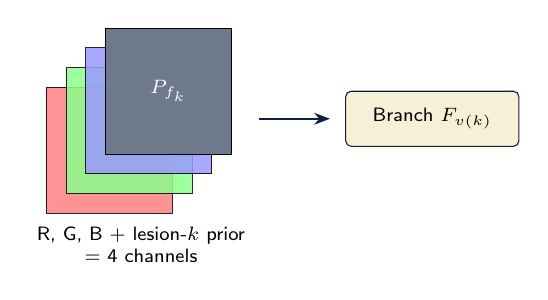
\begin{tikzpicture}[x=1cm,y=1cm]
  \foreach \c/\n/\y in {red!50/R/0, green!45/G/0.25, blue!40/B/0.5}{
    \draw[fill=\c,opacity=0.85] (\y,\y) rectangle ++(1.6,1.6);}
  \draw[fill=navy!60] (0.75,0.75) rectangle ++(1.6,1.6);
  \node[font=\sffamily\scriptsize,text=white] at (1.55,1.55) {$P_{f_k}$};
  \node[font=\sffamily\scriptsize,align=center] at (1.2,-0.4) {R, G, B + lesion-$k$ prior\\= 4 channels};
  \draw[arr] (2.7,1.2) -- (3.6,1.2);
  \node[unet,minimum width=2.2cm] at (4.9,1.2) {Branch $F_{v(k)}$};
\end{tikzpicture}
\end{center}

The paper brands this the ``\emph{multi-perspective lesion navigation strategy}''. Giving a simple
operation a memorable name is a common (and legitimate) writing device: it makes the idea easy to
cite. A variant called HEL-Net-A, which feeds \emph{all four} priors to every branch, was also tested
(Table~8); one prior per branch worked better on IDRiD (about $+0.87$ mIoU / $+0.71$ mDice).

\begin{recap}
Each specialist receives the image \emph{plus} a ``look here'' map for its own lesion.
\end{recap}

% =====================================================================
\section{Step 4 --- The heterogeneous specialist branches}
% =====================================================================
Each branch $k$ produces a full four-class prediction $P_{v(k)} = F_{v(k)}(x_{v(k)})$ (Eq.~10).
The assignment of backbones is:
\begin{center}
\small
\begin{tabular}{@{}llll@{}}
\toprule
Branch & Specialises in & Backbone & Parameters (approx.)\\
\midrule
Net1 & EX (hard exudates) & U-Net & 13.40\,M\\
Net2 & SE (soft exudates) & Mamba-UNet & 19.12\,M\\
Net3 & HE (haemorrhages) & Mamba-UNet & 19.12\,M\\
Net4 & MA (microaneurysms) & U-Net & 13.40\,M\\
\bottomrule
\end{tabular}
\end{center}

\textbf{Where does specialisation come from?} Two signals:
\begin{enumerate}
\item the \textbf{prior channel} (\emph{where to look}), and
\item the \textbf{loss weights}, which double the importance of the branch's own lesion (\emph{what to care about}; see Step 7).
\end{enumerate}

\begin{worked}[Counting HEL-Net's parameters]
Stage 1 (Mamba-UNet) $+$ two Mamba-UNet branches $+$ two U-Net branches:
\[
19.12 + 2(19.12) + 2(13.40) = 19.12 + 38.24 + 26.80 = \mathbf{84.16\,M}.
\]
This matches Table~7 \cmark. (The FAB adds only $\approx 20$ parameters --- see Step 5.)
\end{worked}

\begin{careful}[Rationale vs.\ design mismatch]
The introduction says U-Net is used for \emph{small} lesions, yet U-Net is assigned to EX, which are
among the \emph{largest} lesions. The ablation supports the assignment empirically, but the written
reason does not match it. Lesson for your own writing: let the rationale follow the evidence.
\end{careful}

\begin{recap}
Four specialists, two architectures. Specialisation = prior channel + loss emphasis.
\end{recap}

% =====================================================================
\section{Step 5 --- Feature Aggregation Block: the learned vote}
% =====================================================================
\begin{idea}
Each of the 4 branches outputs 4 class maps $\Rightarrow$ 16 maps. For lesion $c$, the FAB takes the
four class-$c$ maps (one from each branch), stacks them, and mixes them with a
$1\times1$ convolution (Eq.~11):
\[
X_{c} = w_{c,1}P_{1,c} + w_{c,2}P_{2,c} + w_{c,3}P_{3,c} + w_{c,4}P_{4,c} + b_c ,\qquad
Y_{out}=\mathrm{Concat}(X_1,\dots,X_4).
\]
\end{idea}

\begin{center}
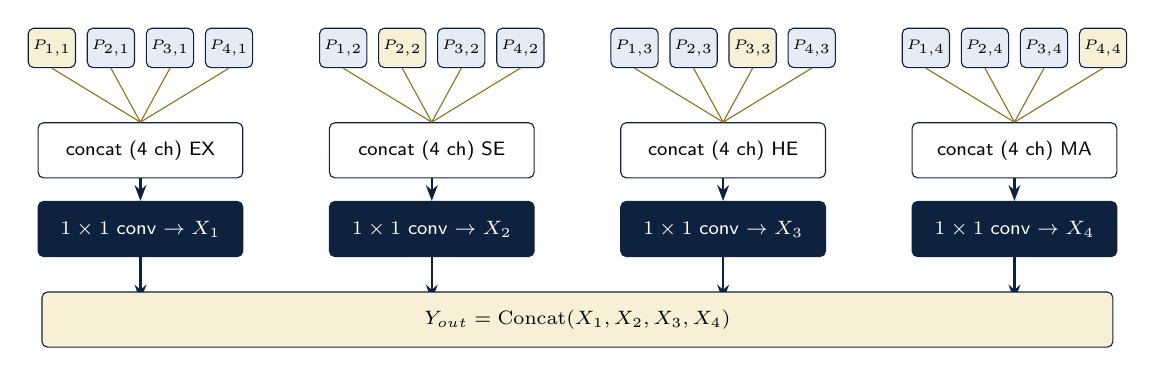
\begin{tikzpicture}[x=1cm,y=1cm]
  \foreach \c/\name [count=\j] in {EX/EX,SE/SE,HE/HE,MA/MA}{
    \pgfmathsetmacro{\x}{(\j-1)*3.7}
    \foreach \b in {1,2,3,4}{
      \pgfmathsetmacro{\xx}{\x+(\b-1)*0.75}
      \ifnum\b=\j
        \node[unet,minimum width=6mm,minimum height=5mm,inner sep=1pt] (p\j\b) at (\xx,0) {\tiny$P_{\b,\j}$};
      \else
        \node[mamba,minimum width=6mm,minimum height=5mm,inner sep=1pt] (p\j\b) at (\xx,0) {\tiny$P_{\b,\j}$};
      \fi
    }
    \node[blk,minimum width=2.6cm] (cc\j) at (\x+1.125,-1.3) {concat (4 ch) \name};
    \node[dark,minimum width=2.6cm] (cv\j) at (\x+1.125,-2.3) {$1\times1$ conv $\rightarrow X_{\j}$};
    \foreach \b in {1,2,3,4}{\draw[gold!70!black] (p\j\b.south) -- (cc\j.north);}
    \draw[arr] (cc\j)--(cv\j);
    \draw[arr] (cv\j.south) -- ++(0,-0.55);
  }
  \node[unet,minimum width=13.6cm] at (6.675,-3.45) {$Y_{out}=\mathrm{Concat}(X_1,X_2,X_3,X_4)$};
\end{tikzpicture}
\end{center}

\begin{analogy}[Weighted voting]
For haemorrhages, the chairperson might learn: ``trust the HE specialist $60\%$, the SE specialist
$20\%$, the others $10\%$ each.'' For microaneurysms the weights would be different. The FAB
\emph{learns} these trust levels from data.
\end{analogy}

\begin{worked}[FAB on one pixel]
Suppose at one pixel the four branches give HE probabilities $0.9,\ 0.4,\ 0.8,\ 0.2$ and the learned
weights are $w=(0.1,\,0.2,\,0.6,\,0.1)$, $b=0$:
\[
X_{\text{HE}} = 0.1(0.9)+0.2(0.4)+0.6(0.8)+0.1(0.2)=0.09+0.08+0.48+0.02=0.67 .
\]
\textbf{Size of the FAB:} $4$ weights $+\,1$ bias $=5$ per class, $\times 4$ classes $=\mathbf{20}$
parameters. Tiny, yet the ablation credits it with $+1.44$ mAUPR on IDRiD.
\end{worked}

\begin{careful}
The text claims the FAB improves ``all four lesion types''. True on IDRiD, but on DDR the SE score
\emph{drops} ($41.27\rightarrow39.63$), and the reported DDR mAUPR gain ($+1.66$) recomputes to
$46.22-45.07=+1.15$.
\end{careful}

% =====================================================================
\section{Step 6 --- Inside Mamba-UNet and the VSS block}
% =====================================================================
\subsection{The architecture}
\begin{center}
\small
\begin{tabular}{@{}lll@{}}
\toprule
Stage & Resolution & Channels\\
\midrule
Patch embedding ($4\times4$) & $H/4\times W/4$ & $C$\\
Encoder 1--4 (2 VSS blocks each + patch merging) & $1/4,\ 1/8,\ 1/16,\ 1/32$ & $C,\,2C,\,4C,\,8C$\\
Decoder (2 VSS blocks each + patch expanding + skips) & back to $1/4$ & $4C,\,2C,\,C$\\
Linear projection & $H\times W$ & number of classes\\
\bottomrule
\end{tabular}
\end{center}
It is a U-Net in which every convolutional block is replaced by a \textbf{Visual State Space (VSS)}
block.

\subsection{The VSS block}
\begin{center}
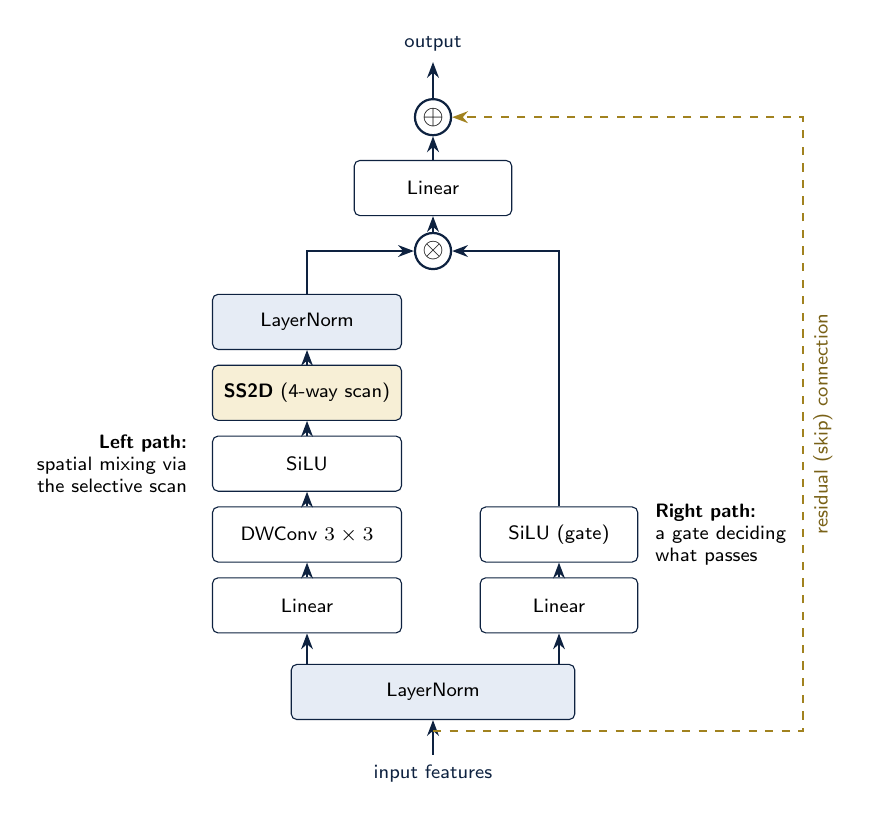
\begin{tikzpicture}[x=1cm,y=1cm]
  \node[mamba,minimum width=3.6cm] (ln0) at (0,0) {LayerNorm};
  % left path
  \node[blk,minimum width=2.4cm] (lin1) at (-1.6,1.1) {Linear};
  \node[blk,minimum width=2.4cm] (dw)   at (-1.6,2.0) {DWConv $3\times3$};
  \node[blk,minimum width=2.4cm] (silu1)at (-1.6,2.9) {SiLU};
  \node[unet,minimum width=2.4cm] (ss2d)at (-1.6,3.8) {\textbf{SS2D} (4-way scan)};
  \node[mamba,minimum width=2.4cm] (ln1) at (-1.6,4.7) {LayerNorm};
  % right path
  \node[blk,minimum width=2.0cm] (lin2) at (1.6,1.1) {Linear};
  \node[blk,minimum width=2.0cm] (silu2)at (1.6,2.0) {SiLU (gate)};
  % merge
  \node[circle,draw=navy,thick,inner sep=1pt] (mul) at (0,5.6) {$\otimes$};
  \node[blk,minimum width=2.0cm] (lin3) at (0,6.4) {Linear};
  \node[circle,draw=navy,thick,inner sep=1pt] (add) at (0,7.3) {$\oplus$};
  \draw[arr] (0,-0.8) node[below,font=\sffamily\scriptsize]{input features} -- (ln0);
  \draw[arr] (ln0.north -| lin1) -- (lin1);
  \draw[arr] (ln0.north -| lin2) -- (lin2);
  \draw[arr] (lin1)--(dw); \draw[arr] (dw)--(silu1); \draw[arr] (silu1)--(ss2d); \draw[arr] (ss2d)--(ln1);
  \draw[arr] (lin2)--(silu2);
  \draw[arr] (ln1.north) |- (mul.west);
  \draw[arr] (silu2.north) |- (mul.east);
  \draw[arr] (mul)--(lin3); \draw[arr] (lin3)--(add);
  \draw[arr] (add) -- (0,8.0) node[above,font=\sffamily\scriptsize]{output};
  \draw[darr] (0,-0.5) -- (4.7,-0.5) |- (add.east);
  \node[font=\sffamily\scriptsize,gold!60!black,rotate=90] at (4.95,3.4) {residual (skip) connection};
  \node[font=\sffamily\scriptsize,align=right,anchor=east] at (-3.0,2.9)
     {\textbf{Left path:}\\spatial mixing via\\the selective scan};
  \node[font=\sffamily\scriptsize,align=left,anchor=west] at (2.7,2.0)
     {\textbf{Right path:}\\a gate deciding\\what passes};
\end{tikzpicture}
\end{center}

\textbf{SS2D (2-D selective scan)} is the heart. An image is 2-D but Mamba reads 1-D sequences, so the
feature map is unrolled in \textbf{four directions} (left$\to$right, right$\to$left, top$\to$bottom,
bottom$\to$top), each sequence is scanned by a selective SSM, and the four results are merged. This
removes the bias of reading the image in only one direction.

\subsection{The state-space model --- step by step}
\textbf{(a) Continuous form (Eq.~12).} A hidden state $h(t)$ evolves with the input $x(t)$:
\[
h'(t) = A\,h(t) + B\,x(t),\qquad y(t) = C\,h(t).
\]
\textbf{(b) Discretise (Eq.~13).} Computers work in steps of size $\Delta$. Holding $x$ constant during
a step (``zero-order hold''):
\[
\bar A = e^{\Delta A},\qquad \bar B = (\Delta A)^{-1}\big(e^{\Delta A}-I\big)\,\Delta B,\qquad
h_t=\bar A\,h_{t-1}+\bar B\,x_t,\qquad y_t = C\,h_t .
\]
\textbf{(c) Selective = input-dependent.} Mamba makes $B$, $C$ and $\Delta$ \emph{functions of the
input}, so the model can decide, token by token, what to remember and what to forget. It is still
computed by a parallel scan with cost $\mathcal{O}(L)$.

\begin{worked}[A 1-D SSM with three numbers]
Take a scalar state with $A=-1$, $B=1$, $C=1$, step $\Delta=0.5$.
\[
\bar A = e^{-0.5}=0.607,\qquad \bar B=\frac{e^{-0.5}-1}{-0.5}\times 0.5 = 1-e^{-0.5}=0.393 .
\]
Feed the input sequence $x=[1,\,0,\,0]$ (a single ``spike''), starting with $h_0=0$:
\[
h_1=0.393,\qquad h_2=0.607\times0.393=0.239,\qquad h_3=0.607\times0.239=0.145 .
\]
The state \textbf{remembers} the spike and \textbf{fades} it gradually. A larger $\Delta$ would forget
faster; a smaller $\Delta$ would remember longer. \emph{Selective} Mamba learns to choose $\Delta$ per
token --- e.g.\ remember lesion-like patches longer, forget plain background quickly.
\end{worked}

\begin{careful}[Notation slips in the paper]
Eq.~13 is printed as $y_t=Cx_t$; it should be $y_t=Ch_t$. The convolution kernel ``$K$'' is mentioned
but never defined (it is $\bar K = (C\bar B,\,C\bar A\bar B,\,\dots,\,C\bar A^{L-1}\bar B)$). The
symbol $C$ is also reused for RGB channels, number of classes and the SSM output matrix.
\end{careful}

\begin{recap}
Mamba-UNet = U-Net built from VSS blocks. VSS = gated block around SS2D. SS2D = four-direction
selective scan. The SSM keeps a fading memory whose fading rate is learned per token.
\end{recap}

% =====================================================================
\section{Step 7 --- Training with triple supervision}
% =====================================================================
\begin{idea}
The network is corrected at \textbf{three points} (Eq.~14):
\[
\mathcal{L}_{seg} = \underbrace{\mathcal{L}_M}_{\text{stage 1}} \;+\;
\underbrace{\textstyle\sum_{k=1}^{4}\mathcal{L}_S^{k}}_{\text{each branch}} \;+\;
\underbrace{\mathcal{L}_O}_{\text{fused output}} .
\]
$\mathcal{L}_M$ and $\mathcal{L}_S^k$ are weighted cross-entropy; $\mathcal{L}_O$ is weighted binary
cross-entropy.
\end{idea}

\begin{analogy}
A teacher who checks the rough draft, each chapter, and the final essay --- rather than only the final
essay --- gives feedback that reaches every part of the work.
\end{analogy}

\subsection*{The weight table (Table 1)}
\begin{center}
\small
\begin{tabular}{@{}llccccc@{}}
\toprule
Weight & Applies to & EX & SE & HE & MA & BG\\
\midrule
$w^M$ & stage 1 & 1 & 2 & 1 & 2 & 0.1\\
$w^S_{c,1}$ & branch EX & \textbf{2} & 2 & 1 & 2 & 0.1\\
$w^S_{c,2}$ & branch SE & 1 & \textbf{4} & 1 & 2 & 0.1\\
$w^S_{c,3}$ & branch HE & 1 & 2 & \textbf{2} & 2 & 0.1\\
$w^S_{c,4}$ & branch MA & 1 & 2 & 1 & \textbf{4} & 0.1\\
$w^O$ & fused output & 10 & 40 & 10 & 40 & --\\
\bottomrule
\end{tabular}
\end{center}

\textbf{How to read it.} Start from base weights (EX 1, SE 2, HE 1, MA 2, background 0.1). The rare
classes SE and MA get twice the weight. For branch $k$, multiply \emph{its own} lesion's weight by
$T=2$ (bold entries). Background gets $0.1$ so the 97.8\% of empty pixels do not dominate.

\begin{worked}[Why weight the loss?]
Imagine 1000 background pixels and 1 MA pixel, each with error 1. Unweighted loss: background
contributes $1000$, MA contributes $1$ --- the network ignores MA. With weights $0.1$ and $4$:
background $=100$, MA $=4$. Still small, but $40\times$ more influential than before. Weights shift
attention toward what matters clinically.
\end{worked}

\begin{careful}[Training schedule is ambiguous]
The paper says the branches are ``trained independently'' and that the ensemble is ``jointly
optimised''. Whether Stage 1 is frozen, detached, or trained end-to-end with the branches is never
stated. A short algorithm box would remove the ambiguity.
\end{careful}

\subsection*{Training settings}
\begin{center}
\small
\begin{tabular}{@{}ll@{}}
\toprule
Pre-processing & CLAHE (clip 2, grid 8), resize to $800\times800$\\
Augmentation & rotation $\pm20^\circ$, flips, colour jitter, Poisson blending\\
Optimiser & Adam, lr $2\times10^{-4}$, $\beta_1=0.5$, $\beta_2=0.999$\\
Schedule & lr $\times0.9$ every 100 epochs, 400 epochs, batch size 2\\
Hardware & PyTorch, one RTX A6000 (48\,GB)\\
\bottomrule
\end{tabular}
\end{center}

% =====================================================================
\section{Step 8 --- Reading the results}
% =====================================================================
\subsection{Headline comparison}
\begin{center}
\small
\begin{tabular}{@{}llccc@{}}
\toprule
Dataset & Metric & HEL-Net & Strongest other & $\Delta$ (points)\\
\midrule
IDRiD & mIoU & 51.99 & 49.94 (M2MRF) & \textcolor{okgreen}{$+2.05$}\\
IDRiD & mDice & 67.40 & 65.71 (M2MRF) & \textcolor{okgreen}{$+1.69$}\\
IDRiD & mAUPR & 69.52 & 68.79 (HACDR-Net) & \textcolor{okgreen}{$+0.73$}\\
DDR & mIoU & 39.05 & 33.70 (HACDR-Net) & \textcolor{okgreen}{$+5.35$}\\
DDR & mDice & 55.25 & 49.30 (HACDR-Net) & \textcolor{okgreen}{$+5.95$}\\
DDR & mAUPR & 46.22 & 50.36 (HACDR-Net) & \textcolor{badred}{$-4.14$}\\
\bottomrule
\end{tabular}
\end{center}

\begin{worked}[Verify a mean yourself]
IDRiD per-lesion Dice for HEL-Net: EX 80.85, SE 73.44, HE 66.32, MA 48.98.
\[
\text{mDice}=\frac{80.85+73.44+66.32+48.98}{4}=\frac{269.59}{4}=67.40\ \cmark
\]
Also EX: IoU $=0.8085/(2-0.8085)=67.86\%$, exactly the reported EX IoU \cmark.
\end{worked}

\subsection{Per-lesion ranking on IDRiD}
\begin{center}
\small
\begin{tabular}{@{}lcccc@{}}
\toprule
Metric & EX & SE & HE & MA\\
\midrule
IoU & \cmark\ 1st & \cmark\ 1st & 2nd & \cmark\ 1st\\
Dice & \cmark\ 1st & \cmark\ 1st & 2nd & \cmark\ 1st\\
AUPR & \cmark\ 1st & 2nd & \cmark\ 1st & \xmark\ 5th\\
\bottomrule
\end{tabular}
\end{center}
MA --- the tiniest lesion --- remains the hardest: MA Dice is only $48.98\%$. Note also the paper's
other evidence: mean $\pm$ SD across images, $t$-test $p$-values, box plots, PR curves and
qualitative overlays (yellow = correct, red = false positive, green = missed).

\subsection{What the DDR AUPR drop means}
On DDR, HEL-Net is best on Dice/IoU but only about 6th on mAUPR. High Dice with lower AUPR suggests
HEL-Net's advantage comes partly from a well-chosen \emph{threshold} (calibration), not from ranking
every pixel better. This is a good example of why reporting a threshold-free metric matters.

% =====================================================================
\section{Step 9 --- Ablations: what each piece contributes}
% =====================================================================
\begin{idea}
An \emph{ablation} removes or swaps one component to see how much it matters. The key question
is: \textbf{is HEL-Net better because of its design, or just because it is bigger?}
\end{idea}

Variants are named by \emph{Stage-1 backbone -- branch backbones}: ``M'' = Mamba-UNet, ``U'' = U-Net.
For example M-U4 means Mamba Stage 1 with four U-Net branches; HEL-Net is effectively M-U2M2.

\begin{center}
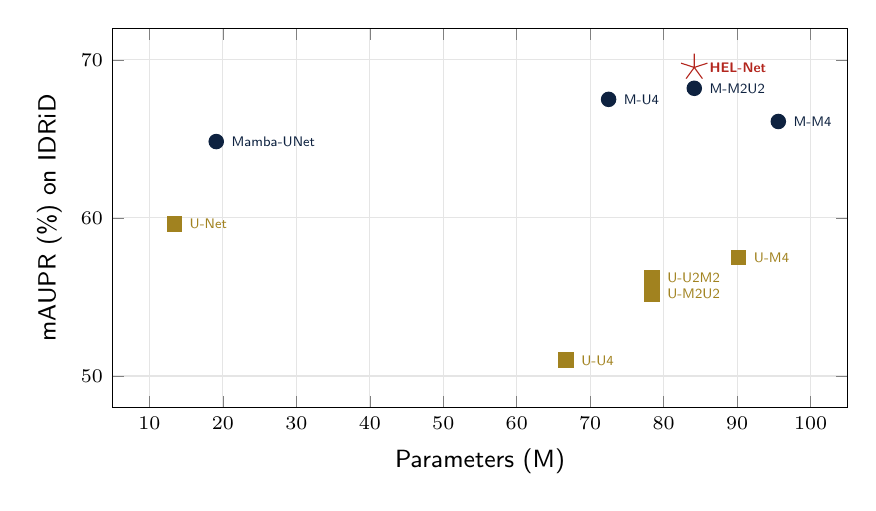
\begin{tikzpicture}
\begin{axis}[
  width=0.9\linewidth, height=6.4cm,
  xlabel={Parameters (M)}, ylabel={mAUPR (\%) on IDRiD},
  xmin=5, xmax=105, ymin=48, ymax=72,
  grid=major, grid style={gray!20},
  label style={font=\sffamily\small}, tick label style={font=\sffamily\scriptsize},
  nodes near coords, point meta=explicit symbolic,
  every node near coord/.append style={font=\sffamily\tiny,anchor=west,xshift=2pt},
]
\addplot[only marks,mark=*,navy,mark size=2.6pt] coordinates {
  (19.1,64.83) [Mamba-UNet] (72.5,67.5) [M-U4] (84.16,68.2) [M-M2U2] (95.6,66.1) [M-M4]};
\addplot[only marks,mark=square*,gold!80!black,mark size=2.6pt] coordinates {
  (13.4,59.63) [U-Net] (66.7,51.0) [U-U4] (78.4,56.2) [U-U2M2] (78.4,55.2) [U-M2U2] (90.2,57.5) [U-M4]};
\addplot[only marks,mark=star,badred,mark size=5pt] coordinates {(84.16,69.52) [\textbf{HEL-Net}]};
\end{axis}
\end{tikzpicture}
\end{center}
{\small Navy circles: Mamba-UNet Stage 1. Gold squares: U-Net Stage 1. Red star: HEL-Net. Positions
of intermediate variants are approximate, redrawn from the decode.}

\textbf{Three lessons from this plot:}
\begin{enumerate}
\item \textbf{Capacity is not the explanation.} M-M4 has the most parameters but is beaten by smaller
      variants.
\item \textbf{Assignment matters.} HEL-Net and M-M2U2 have \emph{identical} size (84.16\,M); they
      differ only in which lesion gets which backbone --- worth $+1.32$ mAUPR.
\item \textbf{A weak prior poisons the cascade.} Every U-Net-first variant falls \emph{below} a plain
      U-Net. Stage 1 must be strong.
\end{enumerate}
Other ablations: Mamba-UNet beats U-Net alone by $5.20$ mAUPR ($64.83-59.63$); the FAB adds
$+1.44$ mAUPR on IDRiD; the branch weight multiplier $T=2$ was tuned in Table~11.

\subsection*{The cost}
HEL-Net needs $484.86$ GFLOPs and runs at $6.27$ images per second --- $1.28\times$ HRNetV2,
$1.37\times$ M2MRF and $2.65\times$ HACDR-Net in compute, and the slowest of the compared methods.
The paper calls this ``slightly higher''; a reader should judge that wording critically.

% =====================================================================
\section{Step 10 --- Thinking like a reviewer}
% =====================================================================
\subsection{Strengths}
\begin{itemize}
\item A clear, well-motivated idea: match backbones to lesion characteristics and guide them with priors.
\item A rich evidence package: two datasets, SD, $p$-values, box plots, PR curves, four ablations,
      complexity analysis.
\item The architecture-combination ablation with parameter counts genuinely separates design from size.
\item An honest limitation (computational cost) and concrete future work.
\end{itemize}

\subsection{Weaknesses}
\begin{enumerate}
\item \textbf{Test-set tuning.} IDRiD has no validation split, so $T$ and thresholds seem chosen on the
      27 test images.
\item \textbf{Statistics.} The test type is unspecified, $n=27$, and 42 $p$-values are reported with no
      multiple-comparison correction.
\item \textbf{Mixed baselines.} Some baseline means are copied from earlier papers while SDs come from
      re-runs.
\item \textbf{Novelty overlap.} Poisson augmentation and Mamba-UNet are adapted; the novelty is the
      combination.
\item \textbf{Reproducibility.} No code, no seeds, patch size and width $C$ unspecified, $\beta$ missing.
\item \textbf{Presentation.} More than ten numeric or labelling inconsistencies (some listed below).
\end{enumerate}

\begin{worked}[Multiple comparisons in one line]
With $42$ tests at $\alpha=0.05$, about $42\times0.05\approx2$ would look ``significant'' by pure chance
even if nothing were real. The Bonferroni correction uses $\alpha=0.05/42\approx0.0012$. Under it,
only 16 of the 39 originally-significant entries survive, and against the two strongest baselines
just one metric each.
\end{worked}

\subsection{A sample of the number audit}
\begin{center}
\small
\begin{tabularx}{\linewidth}{@{}l X X c@{}}
\toprule
Where & Claim in text & Recomputed & OK?\\
\midrule
\S4.4.1 IDRiD & MA AUPR is ``second-best'' & ranks 5th (45.70 vs 48.80, 46.94, 46.27, 46.01) & \xmark\\
\S4.4.1 DDR & MA Dice gain ``more than 2.26\%'' & $39.86-27.67=12.19$ & \xmark\\
Table 3 & Twins-SVT-B mAUPR 63.84 & implies a digit swap (63.12 vs 36.12) & \xmark\\
\S4.5.1 & Mamba-UNet beats U-Net by 5.2 mAUPR & $64.83-59.63=5.20$ & \cmark\\
Table 7 & HEL-Net 84.16\,M params & $19.12+2(19.12)+2(13.40)$ & \cmark\\
\S4.5.4 & cost ``slightly higher'' & up to $2.65\times$ GFLOPs, slowest & \xmark\\
\bottomrule
\end{tabularx}
\end{center}
None of these changes the main conclusion on IDRiD, but each is the kind of detail a careful reviewer
uses to question everything else.

\subsection{Questions a reviewer would ask}
\begin{enumerate}
\item What does a single network with $\approx84$\,M parameters achieve (capacity control)?
\item Is Stage 1 frozen or trained jointly? Is its output detached before Data Fusion?
\item How is the Dice threshold chosen, and on which split?
\item How sensitive are results to resizing ($2848\times4288\rightarrow800\times800$ distorts shape and
      shrinks MAs by $3.6$--$5.4\times$)?
\item Can results be given as mean $\pm$ SD over at least three random seeds?
\end{enumerate}

% =====================================================================
\section{AI ethics corner --- what this paper teaches beyond accuracy}
% =====================================================================
\begin{ethics}[1. Honest evaluation is an ethical duty in medical AI]
Tuning hyper-parameters or thresholds on the \emph{test} set makes a model look better than it will be
on new patients. In medicine, an over-optimistic number can translate into missed disease. Good
practice: train / validation / test splits, report how every choice was made, and keep the test set
untouched until the end.
\end{ethics}

\begin{ethics}[2. Reproducibility and openness]
Data ``on request'' and no released code mean other groups cannot verify the claims. Releasing code,
seeds and exact settings is part of scientific accountability --- especially when results may influence
clinical tools.
\end{ethics}

\begin{ethics}[3. Statistics and the temptation of selective claims]
Reporting 42 $p$-values and highlighting only the favourable ones, without correction, is a mild form
of \emph{p-hacking}. The ethical habit is to pre-state which comparisons matter and correct for
multiplicity.
\end{ethics}

\begin{ethics}[4. Generalisation and fairness]
IDRiD (81 images) and DDR (757 images) come from specific populations, cameras and clinics. A model
trained there may perform worse on other ethnic groups, cameras or image qualities. Before clinical use
one needs external validation across diverse populations and subgroup analysis.
\end{ethics}

\begin{ethics}[5. Honest language about cost and novelty]
Calling a $2.65\times$ compute increase ``slightly higher'', or claiming ``for the first time'' without a
hedge, nudges readers toward a rosier view. Precise language is part of research integrity. The cost
also matters for fairness: heavy models are harder to deploy in low-resource clinics where DR screening
is most needed.
\end{ethics}

\begin{ethics}[6. Synthetic data needs care]
Poisson-blended lesions are \emph{synthetic} medical findings. They must never leak into test sets, and
their anatomical realism should ideally be checked by clinicians, so the model does not learn shortcuts
from artefacts.
\end{ethics}

% =====================================================================
\section{Key takeaways}
% =====================================================================
\begin{center}
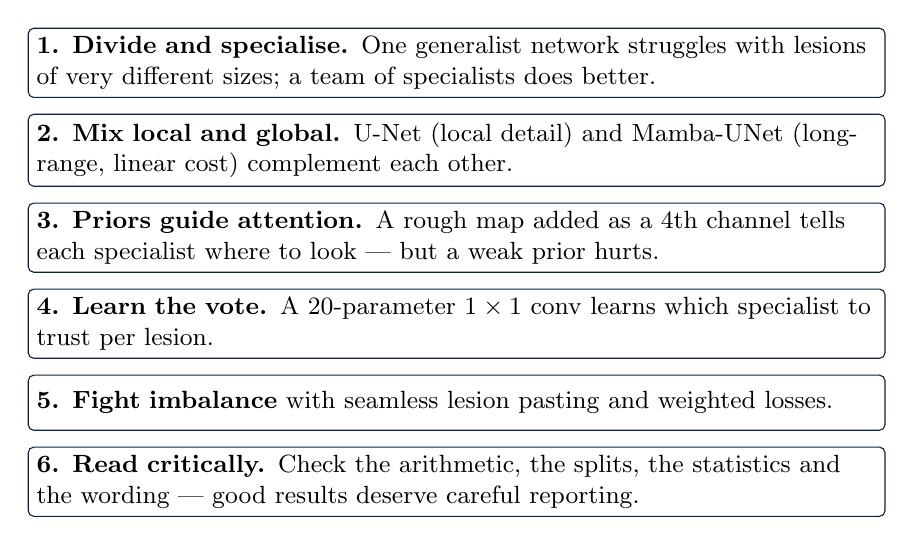
\begin{tikzpicture}[node distance=2mm]
\node[blk,text width=0.88\linewidth,align=left,font=\small] (a)
 {\textbf{1. Divide and specialise.} One generalist network struggles with lesions of very different
 sizes; a team of specialists does better.};
\node[blk,text width=0.88\linewidth,align=left,font=\small,below=of a] (b)
 {\textbf{2. Mix local and global.} U-Net (local detail) and Mamba-UNet (long-range, linear cost)
 complement each other.};
\node[blk,text width=0.88\linewidth,align=left,font=\small,below=of b] (c)
 {\textbf{3. Priors guide attention.} A rough map added as a 4th channel tells each specialist where
 to look --- but a weak prior hurts.};
\node[blk,text width=0.88\linewidth,align=left,font=\small,below=of c] (d)
 {\textbf{4. Learn the vote.} A 20-parameter $1\times1$ conv learns which specialist to trust per lesion.};
\node[blk,text width=0.88\linewidth,align=left,font=\small,below=of d] (e)
 {\textbf{5. Fight imbalance} with seamless lesion pasting and weighted losses.};
\node[blk,text width=0.88\linewidth,align=left,font=\small,below=of e] (f)
 {\textbf{6. Read critically.} Check the arithmetic, the splits, the statistics and the wording ---
 good results deserve careful reporting.};
\end{tikzpicture}
\end{center}

% =====================================================================
\section{Self-check quiz}
% =====================================================================
\begin{enumerate}
\item Why is pixel accuracy a poor metric for MA segmentation?
\item What exactly is ``Data Fusion'' in HEL-Net?
\item Which lesions are handled by U-Net branches, and which by Mamba-UNet branches?
\item A model has Dice $=0.60$ for a lesion. What is its IoU?
\item How many parameters does the FAB have, and why?
\item Why does Mamba scale better than self-attention on an $800\times800$ image?
\item What does the ablation with U-Net as Stage 1 teach us?
\item In the SSM example, what happens to the memory if $\Delta$ becomes larger?
\item Name two reasons the reported IDRiD numbers might be slightly optimistic.
\item Give one ethical concern about deploying HEL-Net in a rural screening programme.
\end{enumerate}

\subsection*{Answers}
\begin{enumerate}[label=\textbf{\arabic*.}]
\small
\item MA covers only $\approx0.10\%$ of pixels; predicting ``no MA'' everywhere already gives $99.9\%$ accuracy.
\item Concatenating the 3-channel image with the 1-channel Stage-1 prior for that branch's lesion (4 channels in total).
\item U-Net: EX and MA. Mamba-UNet: SE and HE (and Stage 1).
\item $\text{IoU}=0.60/(2-0.60)=0.60/1.40\approx0.429$.
\item 20: for each of 4 classes, 4 weights (one per branch) $+$ 1 bias.
\item $L=40\,000$ tokens; attention costs $\propto L^2=1.6\times10^9$, Mamba $\propto L$.
\item A weak Stage-1 prior misleads all branches: every U-Net-first cascade is worse than a single U-Net.
\item $\bar A=e^{\Delta A}$ gets smaller (with $A<0$), so the state forgets faster.
\item Hyper-parameters/thresholds chosen on the 27-image test set; no multiple-comparison correction; small $n$.
\item Any of: heavy compute ($\approx485$ GFLOPs, 6 FPS) on low-cost hardware; unproven generalisation to
      local populations and cameras; no released code for independent validation.
\end{enumerate}

% =====================================================================
\section{Glossary}
% =====================================================================
\small
\begin{description}[leftmargin=0pt,itemsep=1pt]
\item[Ablation] An experiment that removes or swaps one component to measure its contribution.
\item[AUPR] Area under the precision--recall curve; threshold-free, suited to rare classes.
\item[CLAHE] Contrast-Limited Adaptive Histogram Equalisation: local contrast enhancement.
\item[Cross-entropy (weighted)] Classification loss; weights make rare classes count more.
\item[Data Fusion (DF)] Stacking the image with a lesion prior as a 4th channel.
\item[Dice / IoU] Overlap scores between prediction and ground truth; $\text{IoU}=\text{Dice}/(2-\text{Dice})$.
\item[Ensemble] Combining several models' predictions.
\item[FAB] Feature Aggregation Block: class-wise $1\times1$ convolution that fuses branch outputs.
\item[Heterogeneous] Built from different kinds of models (here U-Net and Mamba-UNet).
\item[Mamba] A selective state-space model with input-dependent parameters and linear cost.
\item[Poisson blending] Seamless pasting that copies gradients inside a region and matches colours on its border.
\item[Prior] A rough map that tells a later network where something probably is.
\item[SS2D] 2-D selective scan: unroll an image in four directions and scan each with an SSM.
\item[SSM] State-space model: $h_t=\bar A h_{t-1}+\bar B x_t$, $y_t=C h_t$.
\item[U-Net] Encoder--decoder CNN with skip connections, the classic segmentation backbone.
\item[VSS block] Visual State Space block: the Mamba building block used inside Mamba-UNet.
\end{description}

\end{document}
